
\documentclass[11pt]{amsbook}
\usepackage[turkish]{babel}

\usepackage{../Ceyhun}	% ------------------------
\usepackage{../amsTurkish}

\usepackage{lipsum}



\begin{document}

% ++++++++++++++++++++++++++++++++++++++
\hPage{ceyhun-007} 
% ++++++++++++++++++++++++++++++++++++++
% =======================================
  kümesindeki düğümlerden biri olan ayrıtların $Ç_1$ den çıkartımına eşittir. 
%I might use \hspace{10cm} for exactly the same page, but I remember that you said "Don't think about such situations
% and just leave it to latex default.". That's why I am leaving it as such.

Tanımladığımız bu işlemleri açıklamak için, Şekil 1.1.6a da gösterilen $Ç_1$ ve $Ç_2$ çizgelerini düşünelim \\
% I don't know the reference of that figure because it is not in my page. Therefore I wrote it by hand, instead of \reffig{fig:...}.

\begin{figure}[htb]
	\centering
	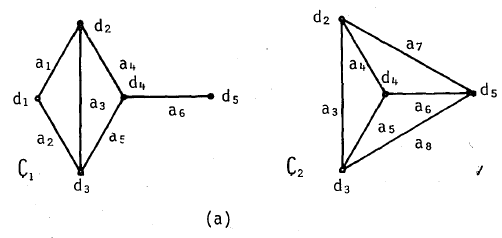
\includegraphics[width=0.95\textwidth]{images/ceyhun-7-fig01}
	\label{fig:1.1.6b}
	
\end{figure}

\begin{figure}[htb]
	\centering
	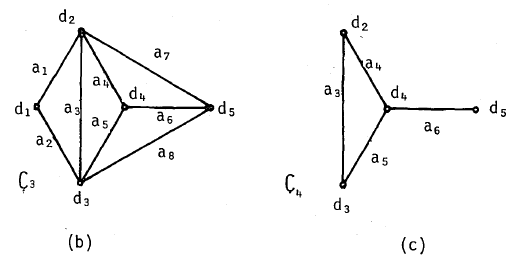
\includegraphics[width=0.95\textwidth]{images/ceyhun-7-fig02}
	\label{fig:1.1.6b}
	
\end{figure}

\end{document}  


